\subsection{Light}

Before getting into the specifics functioning of photosensors or the human vision, one should spend some time reviewing basic things about light itself. 

Light consists of electromagnetic radiation with a dual particle-wave nature. This was pointed out by Einstein in 1905 who theorized that light is composed of discrete quanta called photons with an energy that is inversely proportional to the wavelength of the light, so that $E=hc/\lambda$.
For example a photon that will be seen by our eyes as yellow has a wavelength $λ=555nm$ has $E=2.1eV$ in vacuum.

\begin{figure}[H]
    \centering
    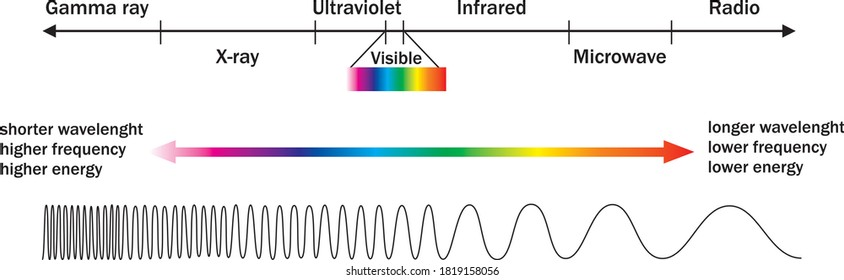
\includegraphics[width=0.7\linewidth]{../../Figures/Light.jpg}
    \caption{Range of photon wavelength. Adapted from somewhere on Google Image.}
    \label{fig:Light}
\end{figure}

\sub{The photon}

Photon is a basic unit of all forms of electromagnetic radiation including light. It has no mass, no electric charge, does not decay spontaneously in vacuum. In vacuum, it moves at speed of light $c$. We can compute the energy $E$ and momentum $P$ of photons: 

\begin{equation}
    E = \frac{h c}{\lambda} = h \nu 
\end{equation}

with frequency of light $\nu = c/\lambda$ in $Hz$.

\begin{equation}
    p = |P| = \frac{h}{\lambda}
\end{equation}

Its energy $E$ and momentum $P$ are related by $E=c\codt p$. (p is magnitude of P). $h$ is Planck's constant. 

\subsubsection{Measuring light: Radiometry and photometry}

\paragraph{Units of light} Measuring light is not done through photon energy, as it is not an informative measure of "illumination" or "brightness". Thought these two are of course related to energy! 
The unit of visible light is the \textbf{Lumen} (noted $lm$). Several measures are derivatives of this unit and are more useful for everyday use. The \textbf{Lux} (noted $lux$) is the measure of visible light on plane surface - it is measured in $lm/m^2$. The \textbf{Candela} (noted $cd$) is also similar to the lux but more appropriate to angular measurements:  it is measured in $lm/steradian$ \footnote{The steradian or square radian is the SI unit of solid angle. It is used in three-dimensional geometry, and is analogous to the radian, which quantifies planar angles. A sphere has $4\pi$ steradian.}. We typically use it to measure the illumination from light sources (e.g. lamp) as light propagates uniformly in all directions. Fun fact: prior to 2018, the basic unit of light was the Candela, but the 26h General conference on Weights and Measures redefined photo metric units. The new definition which took place on may 20th 2019, the lumen \textit{is defined by taking the fixed numerical value of the luminous efficacy of monochromatic radiation of frequency 540 × 1012 Hz, $K_{cd}$, to be 683 when expressed in the unit lm $W^{-1}$}. Understanding the units of light is not straightforward and out of the scope of these lecture notes so let's move on. 
1 Lux of sunlight (because it will be different if you have a different light source as the distribution of wavelenghts emitted might be different) is $\approx 4 \cdot 10^{-3} W/m^2 \approx 10^4$ photons/$ \mu m^2 /s$.

\paragraph{Scene illumination and reflectance}
The typical illumination humans are exposed varies quite a lot: it's about 100 klux in full sunlight and 0.1 lux in moonlight. Light is reflected through surface, at different levels. Opaque materials typically absorb most of the light while the rest reflects most to all of light it receives. The average scene reflectance is about $R \approx 18\% $. 

\paragraph{What do radiometry and photometry mean?} 

\textit{Radiometry} is the science of measurement of \textit{optical radiation at any wavelength}, based simply on physical measurements. Radiant energy cannot be measured quantitatively directly, but must always be converted into some other form such as thermal, electrical, or chemical. 
\textit{Photometry} is the science of measuring visible light in \textit{units that are weighted according to the sensitivity of the human eye}. It is a quantitative science based on a statistical model of the human visual response to light - that is, our perception of light - under carefully controlled conditions.



